\section{}
\paragraph{}\label{answer:72}
آرایه‌ای از یک کلاس مشتق داریم که \lr{\texttt{safe\_stack}} نام دارد. در \lr{\texttt{C++}}، می‌توانید از اشاره‌گری به کلاس پایه \lr{\texttt{(stack*)}} برای اشاره به یک کلاس مشتق \lr{\texttt{(safe\_stack)}} استفاده کنید. سیستم فقط قسمت پایهٔ کلاس را می‌بیند ولی با این حال می‌توانید به آن اشاره کنید.
\begin{center}
    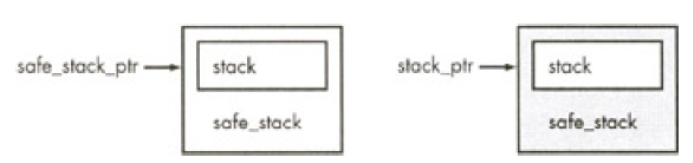
\includegraphics[keepaspectratio,width=0.4\textwidth,height=0.4\textheight]{images/image04.jpg}
\end{center}
حالا یک اشاره‌گر می‌تواند به یک نمونهٔ واحد از یک کلاس یا آرایه‌ای از اشیاء اشاره کند.
\begin{center}
    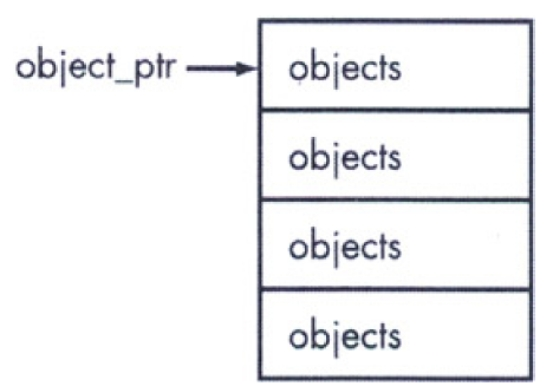
\includegraphics[keepaspectratio,width=0.4\textwidth,height=0.4\textheight]{images/image05.jpg}
\end{center}
بنابراین قوانین زیر را خواهیم داشت:
\begin{enumerate}
    \item اشاره‌گر کلاس پایه می‌تواند به یک شیء مشتق‌شده اشاره کند.
    \item اشاره‌گر به شیء می‌تواند به آرایه‌ای از اشیاء اشاره کند.
\end{enumerate}

از روی این می‌توانیم نتیجه بگیریم:
\begin{enumerate}
    \item یک اشاره‌گر پایه می‌تواند به آرایه‌ای از اشیاء مشتق‌شده اشاره کند.
\end{enumerate}

این غلط است.

مشکل این جاست که آرایه‌ای از اشیاء مشتق‌شده، با آرایه‌ای از اشیاء پایه یکسان نیست.
\begin{center}
    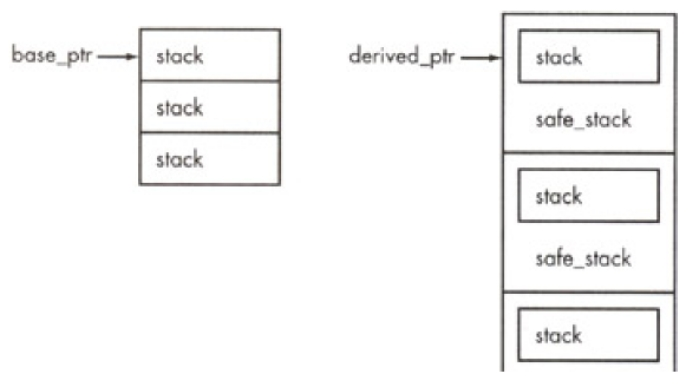
\includegraphics[keepaspectratio,width=0.4\textwidth,height=0.4\textheight]{images/image06.jpg}
\end{center}
بنابراین اگر یک اشاره‌گر پایه را گرفته و آن را به یک آرایه از مشتق‌شده‌ها اشاره دهیم، لایهٔ حافظه غلط خواهد بود.
\begin{center}
    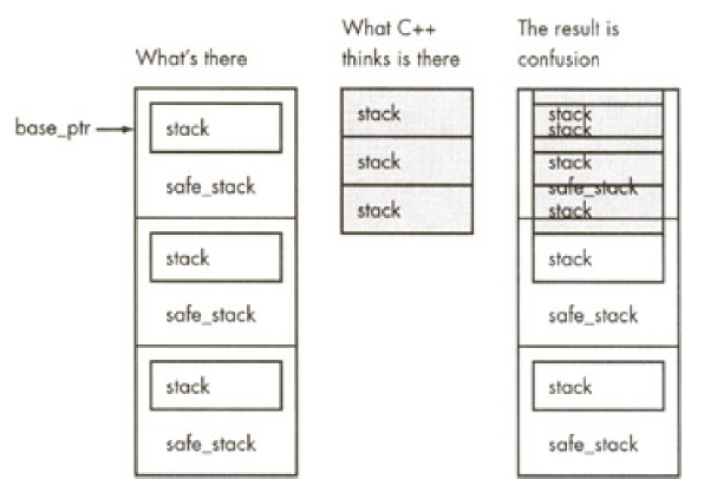
\includegraphics[keepaspectratio,width=0.4\textwidth,height=0.4\textheight]{images/image07.jpg}
\end{center}
از قالب بردار \lr{\texttt{STL}} به جای یک آرایه استفاده کنید. این کار کلی از مشکلات را حل می‌کند. آرایه‌های کلاس پایه را به عنوان پارامتر، ارسال نکنید.